% !TeX root = ../index.tex
\documentclass[../index.tex]{subfiles}

\begin{document}
    \section{Wykład}
        \subsection{Zróżnicowanie gwiazd}
            Gwiazdy mogą się różnić od siebie całkiem znacznie. W obrębie jednego typu gwiazdowego ich parametry są zbliżone, natomiast różnice pomiędzy typami bywają znaczne. Poniższa grafika prezentuje uśrednione wartości (lub przedziały wartości) dla różnych typów gwiazd:
            \begin{center}
                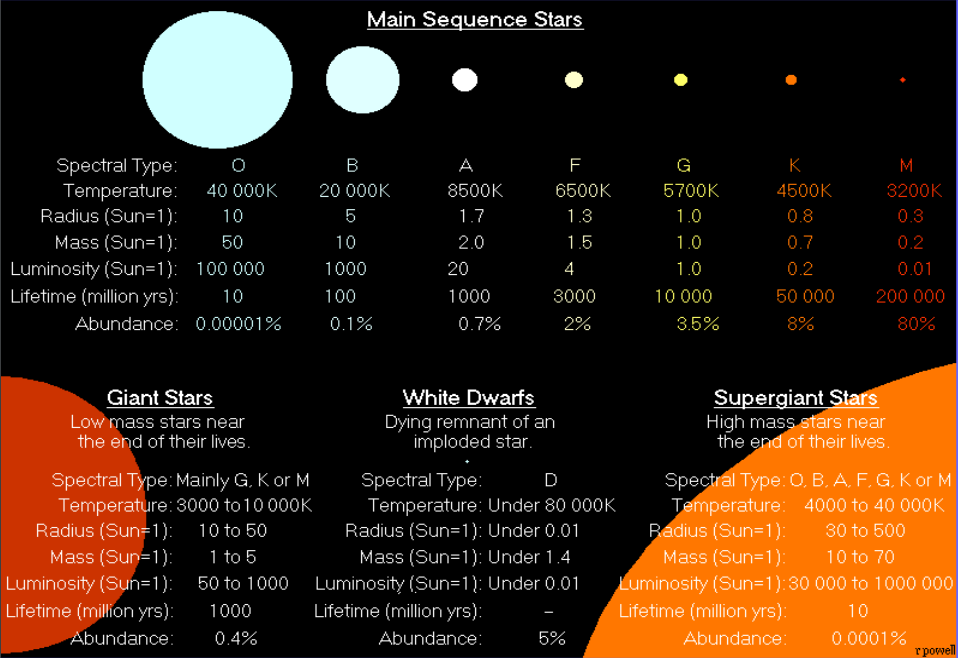
\includegraphics[width=15cm]{images/parametryGwiazd.png}
            \end{center}
            Oprócz znanych parametrów takich jak temperatura, promień masa i jasność wprowadzono także pojęcia \textbf{czasu życia} (czasu przez jaki gwiazda pozostaje w tej postaci) i \textbf{obfitości występowania}. Dokładniejsze dane obejmujące także brązowe karły można znaleźć na wykładzie.
        \subsection{Temperatura fotosfery}
            Do tej pory korzystaliśmy z pojęcia temperatury efektywnej \(T_\text{eff}\),  która była pewną średnią temperaturą pewnej warstwy atmosfery gwiazdy (tej z której dociera do nas światło). Oczywiście temperatura fotosfery ma pewien rozkład, który można zmierzyć. W przypadku słońca można skorzystać z metody pomiaru \textbf{pociemnienia brzegowego} \--- zmierzyć temperatury (zgodnie z prawem Stefana-Boltzmanna) centrum tarczy słońca oraz jej brzegów i na podstawie różnic wyciągać wnioski o rozkładzie temperatury. Poniższy wykres ilustruje spadek temperatury wraz z wysokością względem umownego poziomu zerowego \--- poziomu poniżej którego atmosfera staje się nieprzezroczysta:
            \begin{center}
                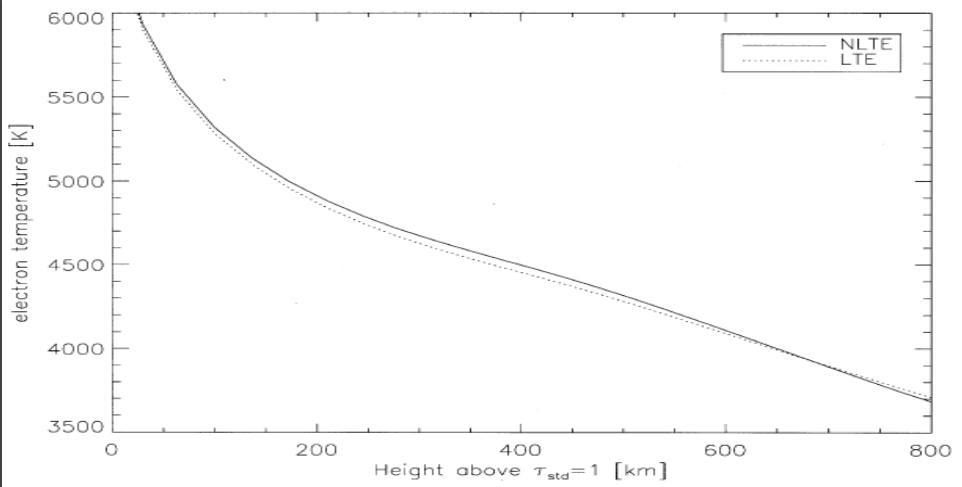
\includegraphics[width=16cm]{images/widmoFotosferySlonca.png}
            \end{center}
            W bardziej ogólnym przypadku aby znaleźć rozkład temperatury musimy skorzystać z \textbf{modelu fotosfery} \--- zestawu najważniejszy parametrów mających wpływ na powstanie widma: temperatura, ciśnienie, gęstość, skład chemiczny i inne. Ponieważ z zarejestrowanego widma nie jesteśmy w stanie odtworzyć fotosfery to problem rozwiązuje się od końca, najpierw tworząc komputerowo \textbf{widmo syntetyczne} tzn. generuje się widmo na podstawie pewnych parametrów. Dalej porównuje się otrzymane widmo z faktycznie zaobserwowanym i koryguje parametry tak, żeby w końcu widmo syntetyczne było wystarczająco bliskie realnemu. Wówczas wprowadzone parametry są bliskie realnym parametrom gwiazdy i na ich podstawie można już opisać fotosferę.
        \subsection{Skład chemiczny gwiazd}
            Dokładna znajomość chemicznego pełni niebagatelną funkcję w modelowaniu fotosfery. \textbf{Metale} w astronomii to wszystkie pierwiastki nie będące wodorem ani helem. Stosunek ilości tych trzech informuje o tym z jakiej materii uformowała się gwiazda, a dokładanie z jak starej materii. Im więcej metali tym gwiazda zbudowana z materii młodszej. Jest tak dlatego, że nie znam innego sposobu na naturalne tworzenie się ciężkich pierwiastków niż reakcja syntezy jądrowej. Także każdy ciężki pierwiastek (jako że wnętrza gwiazdy i fotosfera się nie mieszają) znajdujący się w fotosferze musiał powstać we wnętrzu jakiejś innej, starszej gwiazdy. Gwiazdy obfite w metale, takie jak słońce tworzą \textbf{dysk galaktyczny}, natomiast te o mniejsze zawartości metali tworzą \textbf{halo galaktyczne}:
            \begin{center}
                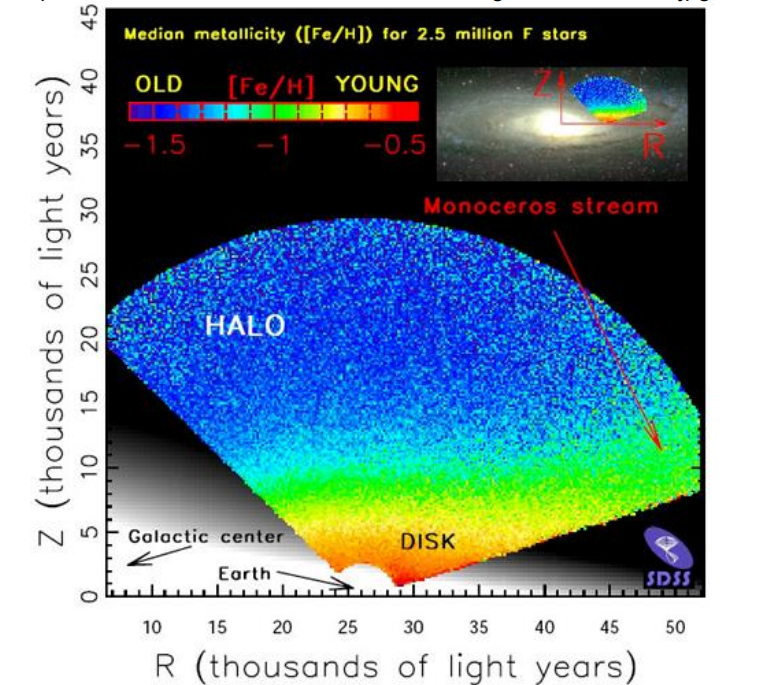
\includegraphics[width=16cm]{images/drogaMlecznaMetale.png}
            \end{center}
            Ostatnio odkryto gwiazdy, w których procentowa zawartość metali jest mniejsza milion razy niż w naszym słońcu. Nazwano je \textbf{First Stars}.
\end{document}